%% Based on techreport.tex template as sent by Erik Burger on 2023-11-20
%% 
%% Karlsruhe Institute of Technology
%% Institute for Program Structures and Data Organization
%% Chair for Software Design and Quality (SDQ)
%%
%% Dr.-Ing. Erik Burger
%% burger@kit.edu
%%
%% See https://sdq.kastel.kit.edu/wiki/Dokumentvorlagen
%%
%% Version 1.0, 2023-11-20

%% Available page modes: oneside, twoside
%% Available languages: english, ngerman
%% Available modes: draft, final (see README)
\documentclass[oneside, nenglish]{sdqtechreport}

%% ---------------------------------
%% | Information about the document |
%% ---------------------------------

%% Name of the group and authors
\author{Paul Buda, Martin Scheuermann, Stephan Schneider, \\
Simon Schütz and Nils Seibert}

%% Title (and possibly subtitle) of the thesis
\title{Design document}

\subtitle{for the Android-App Neptune}

%% You can put a logo in the ``logos'' directory and include it here
%% instead of the SDQ logo
% \grouplogo{myfile}
%% Alternatively, you can disable the group logo
% \nogrouplogo

\date{12.01.2024}

%% For example texts -- please remove in the final version
\usepackage{blindtext}

%% ====================================
%% ====================================
%% ||                                ||
%% || Beginning of the main document ||
%% ||                                ||
%% ====================================
%% ====================================
\begin{document}

%% Set PDF metadata
\setpdf

%% Set the title
\maketitle

%% ------------------------
%% |   Table of Contents  |
%% ------------------------
\tableofcontents

%% -----------------
%% |   Main part   |
%% -----------------
\cleardoublepage

%% -------------------
%% | Example content |
%% -------------------

\chapter{Introduction}
\label{chap:Introduction}

This document summarizes the results of the design phase of the PSE project Neptune.

\chapter{System}
\label{chap:System}

\begin{figure}[h]
    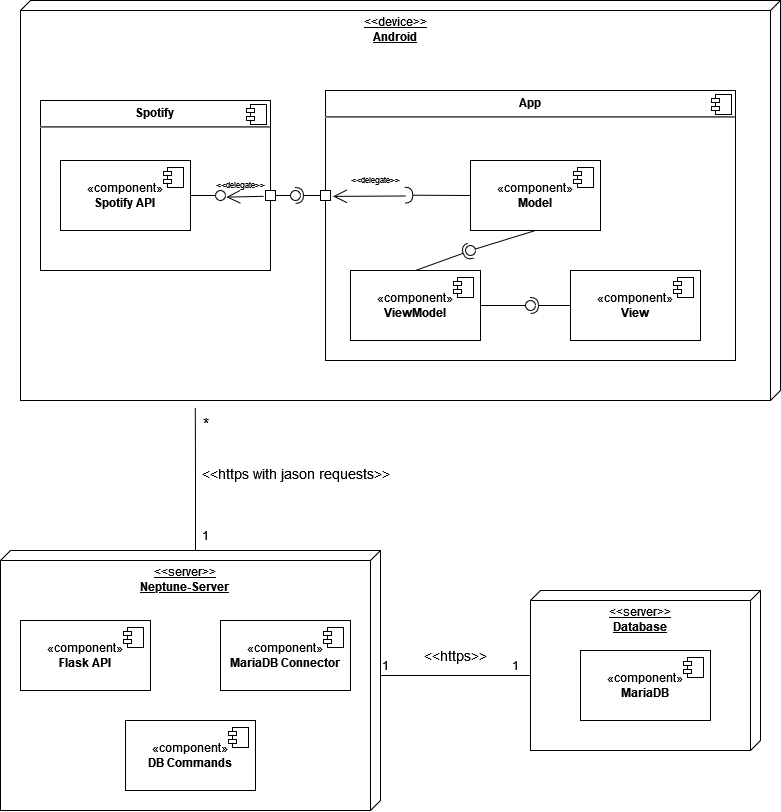
\includegraphics[width = 16cm]{LATEX/Entwurf/Graphics/Component-Diagram.png}
    \caption{Deployment diagram}
    \label{fig:Deployment diagram}
\end{figure}

The entire system of Neptune consits of three pieces: the Android app itself, the Neptune server and a database.

The app makes up the front end part of the system and runs the main application. It can be connected with Spotify via the Spotify API.

The server and the database together form the backend part of the system. The server contains the Neptune sessions and serves as connection between the app and the database. The database stores all relevant data of the sessions.

The server and the app communicate with each other using JSON objects over a https connection. The server and the database also communicate via a https connection.

\chapter{App}
\label{chap:App}

Die Android App wird mithilfe des Entwurfsmusters Model View ViewModel (MVVM) entwickelt. Die hierbei verwendete Programmiersprache ist Kotlin.

\section{Model}
\label{sec:App:Model}

\subsection{session}
\label{sec:App:Model:SessionPacket}
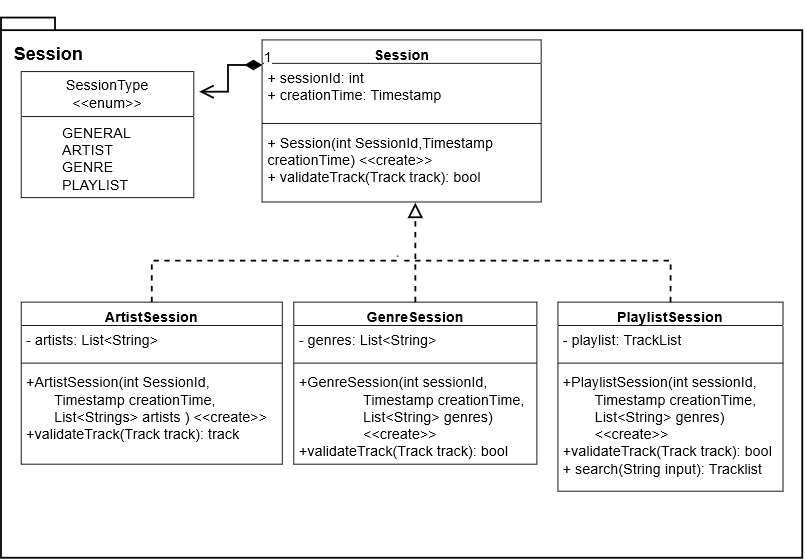
\includegraphics[width = 16cm]{LATEX/Entwurf/Graphics/SessionPacket(1).jpg}
\captionof{figure}{session uml-diagramm}
Holds all the data associated with a session, inheritance is used to implement different types of sessions and there unique requirements.
\subsubsection{Enum SessionType}

Enum to differentiate between the different SessionTypes.

\textbf{values}:
\begin{itemize}
    \item GENERAL
    \item ARTIST
    \item GENRE
    \item PLAYLIST
\end{itemize}

\subsubsection{Class Session}
Represents a Session in General Modus, acts as a parentclass for the other sessionttype classes.

\textbf{attributes:}
\begin{itemize}
    \item public sessionId: int        
    \item public creationTime: Timestamp 
    \begin{itemize}
        \item sessionId and timestamp in combination are unique, and can be used as unique identifer for sessions.
    \end{itemize}
    \item public sessionType: SessionType
\end{itemize}

\textbf{Konstruktoren:}
\begin{itemize}
    \item Session(int sessionId,Timestampt creationTime)
    \begin{itemize}
        \item assigns arguments to attributes.
        \item sets sessionType to SessionType.GENERAL
    \end{itemize}
\end{itemize}
\textbf{Methoden:}
\begin{itemize}
    \item validateTrack(Track track): bool 
    \begin{itemize}
        \item checks if the track is restricted by sessionType.  
        \item returns if True by default, children class override this method to add restriction.
    \end{itemize}
    
\end{itemize}

\subsubsection{Class ArtistSession}
Inherits from Session, represents a Session in Artistmode.

\textbf{attributes:}
\begin{itemize}
    \item private artists: List<String>
    \begin{itemize}
        \item lists all artists, that are allowed in session.
    \end{itemize}
\end{itemize}
\textbf{constructors:}
\begin{itemize}
    \item ArtistSession(int SessionId,TimeStamp timestamp,List<String> artists)
    \begin{itemize}
        \item assigns arguments to attributes.
        \item sets sessionType to SessionType.ARTIST
    \end{itemize}
\end{itemize}

\textbf{methods:}
\begin{itemize}
    \item validateTrack(Track track):bool
    \begin{itemize}
        \item returns True, if the artist of the track is included in artists, false otherwise
    \end{itemize}
\end{itemize}

\subsubsection{Class GenreSession}
Inherits from Session, represents a Session in Genremode.

\textbf{attributes:}
\begin{itemize}
    \item private genre: List<String>
    \begin{itemize}
        \item lists all genres, that are allowed in session.
    \end{itemize}
\end{itemize}
\textbf{constructors:}
\begin{itemize}
    \item ArtistSession(int SessionId,TimeStamp timestamp,List<String> artists)
    \begin{itemize}
        \item assigns arguments to attributes.
        \item sets sessionType to SessionType.GENRE
    \end{itemize}
\end{itemize}

\textbf{methods:}
\begin{itemize}
    \item validateTrack(Track track):bool
    \begin{itemize}
        \item returns True, if the genre of the track is included in genres, false otherwise
    \end{itemize}
\end{itemize}

\subsubsection{Class PlaylistSession}
Inherits from Session, represents a Session in Playlistmode.

\textbf{attributes:}
\begin{itemize}
    \item private playlist: TrackList
    \begin{itemize}
        \item list of all track allowed in the session.
    \end{itemize}
\end{itemize}
\textbf{constructors:}
\begin{itemize}
    \item ArtistSession(int SessionId,TimeStamp timestamp,List<String> artists)
    \begin{itemize}
        \item assigns arguments to attributes.
        \item sets sessionType to SessionType.ARTIST
    \end{itemize}
\end{itemize}

\textbf{methods:}
\begin{itemize}
    \item validateTrack(Track track):bool
    \begin{itemize}
        \item returns True, if the track is included in tracklist, false otherwise
    \end{itemize}
    \item search(String input): Tracklist
    \begin{itemize}
        \item search the tracks in playlist for titles closests to input.
        \item gibt gefundene Tracks als Tracklist zurück.
    \end{itemize}
\end{itemize}

\subsection{backend\_connector}

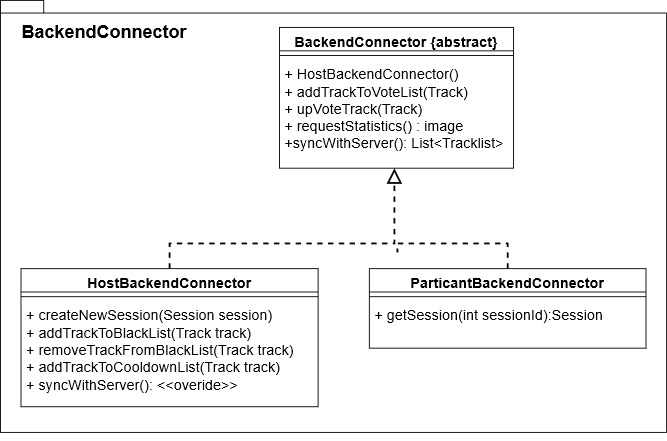
\includegraphics[width = 16cm]{LATEX/Entwurf/Graphics/BackendConnector.jpg}
\captionof{figure}{backend\_connector  uml-diagramm}
Wraps all access to the backend into one class, depending one the role of the user different extensions to the base BackendConnector are added with inheritance. 



 \subsubsection{Class BackendConnector \{abstract\}}
 This abstract class provides the base funcitionality for communicating with the backend, that is needed by all types of user.

 \textbf{attributes:}
 \begin{itemize}
     \item deviceId: String
 \end{itemize}
 \textbf{constructors:}
 \begin{itemize}
     \item BackendConnector():
     \begin{itemize}
         \item hash device data to calculate deviceId and assign it to the attribute.
     \end{itemize}
 \end{itemize}
 \textbf{methods:}
 \begin{itemize}
     \item addTrackToVoteList(Track track) 
     \begin{itemize}
         \item post deviceId and track.Id to https://nep-tune.de:5000/addNewTrack
         \item throws BackendError if returned status is "failed"
     \end{itemize}
     \item upvoteTrack(Track track)
     \begin{itemize}
         \item post deviceId and track.Id to https://nep-tune.de:5000/addUpvoteToTrack
         \item throws BackendError if returned status is "failed"
     \end{itemize}
     \item removeUpvoteFromTrack(Track track)
     \begin{itemize}
         \item post deviceId and track.Id to https://nep-tune.de:5000/removeUpvoteFromTrack
          \item throws BackendError if returned status is "failed"
     \end{itemize}
     \item requestStatistics()
     \begin{itemize}
         \item post deviceID to https://nep-tune.de:5000/getStatatistics
         \item return the jsonresponse from the backend, to the caller for further processing
         \item throws BackendError if returned status is "failed"
     \end{itemize}
     
     \item syncWithServer():
     \begin{itemize}
         \item post deviceId and https://nep-tune.de:5000/getAllTrackData
         \item extract Votelist, BlackList and Cooldownlist from server response, and 
         return them in a List of Tracklists 
         \item throws BackendError if returned status is "failed"
     \end{itemize}
     \item isSessionOpen(Session session): bool
     \begin{itemize}
         \item post deviceId and session.sessionId and session.timestamp to https://nep-tune.de:5000/isSessionOpen
         \item parses backendresponse and returns isOpen field. 
         \item throws BackendError if returned status is "failed" 
     \end{itemize}
 \end{itemize}

 \subsubsection{Class ParticantBackendConnector}
Inherits from BackendConnector, adds methods needed by users in the particicant role.

\textbf{attributes:}
\begin{itemize}
     \item none
\end{itemize}
\textbf{constructors:}
\begin{itemize}
    \item ParticantBackendConnector()
    \begin{itemize}
        \item call super() to invoce BackendConnector()
    \end{itemize}
\end{itemize}
\textbf{methods:}
\begin{itemize}
    \item joinSession(int sessionId): Session
    \begin{itemize}
          \item post deviceId and sessionId to https://nep-tune.de:5000/particantJoinSession
          \item parse the server response into a Sessioninstance that gets returned to the caller.
         \item throws BackendError if returned status is "failed"
     \end{itemize}
     \item leaveSession():
     \begin{itemize}
         \item post deviceId to https://nep-tune.de:5000/particiantLeaveSession
         \item throws BackendError if returned status is "failed"
     \end{itemize}
\end{itemize}

\subsubsection{Class HostBackendConnector}
Inherits from BackendConnector, adds methods needed by users in the host role.

\textbf{attributes:}
\begin{itemize}
     \item none
\end{itemize}
\textbf{constructors:}
\begin{itemize}
    \item HostBackendConnector()
    \begin{itemize}
        \item call super() to invoce BackendConnector()
    \end{itemize}
\end{itemize}
\textbf{methods:}
\begin{itemize}
    \item createNewSession(Session session):
    \begin{itemize}
        \item post deviceId and session data to https://nep-tune.de:5000/createNewSession
        \item sets session.creationTime to the timestamp returned from the server
        \item throws BackendError if returned status is "failed"
    \end{itemize}
    addTrackToBlockList(Track track):
    \begin{itemize}
        \item post deviceId and track.ID with "blocked" = true to https://nep-tune.de:5000/setBlockTrack
        \item throws BackendError if returned status is "failed"
    \end{itemize}
    removeTrackFromBlockList(Track track):
    \begin{itemize}
        \item post deviceId and track.ID  with "blocked" = false to https://nep-tune.de:5000/
        \item throws BackendError if returned status is "failed"
    \end{itemize}
    
\end{itemize}

\subsection{track}
\begin{center}
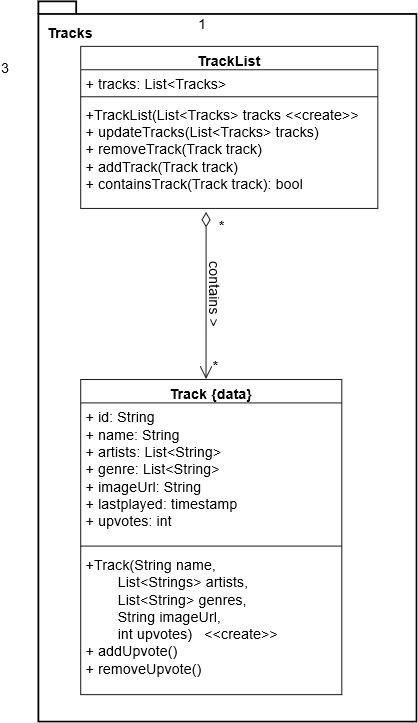
\includegraphics[width = 7cm]{LATEX/Entwurf/Graphics/Track.jpg}
\end{center}
\captionof{figure}{track uml-diagramm}

\subsubsection{class Track}
Holds all data associated with a Track, and provides methods to change the upvote count.

\textbf{attributes:}
\begin{itemize}
    \item id: String {unique}
    \begin{itemize}
        \item unique id provided by the spotifyapi.
    \end{itemize}
    \item name: String
    \begin{itemize}
        \item name that is displayed to the user.
    \end{itemize}
    \item artists: List<String>
    \begin{itemize}
        \item list of all artists associated with this track.
    \end{itemize}
    \item genres: List<String>
    \begin{itemize}
         \item list of all genres associated with this track.
    \end{itemize}
    \item imageUrl: String
    \begin{itemize}
        \item url of the image belonging to the track.
    \end{itemize}
    \item lastPlayed: timeStamp
    \begin{itemize}
        \item Timestamp of the last time the track was played.
        \item zero, if the track hasn´t been played yet.
    \end{itemize}
\end{itemize}
\textbf{constructors:}
\begin{itemize}
    \item Track(String name,List<Strings> artists,List<String> genres,String imageUrl,int upvotes)
    \begin{itemize}
        \item assign all the arguments to attributes
    \end{itemize}
\end{itemize}
\textbf{methods:}
\begin{itemize}
    \item addUpvote()
    \begin{itemize}
        \item adds one to upvote counter.
    \end{itemize}
    \item removeUpvote()
    \begin{itemize}
        \item subtract one from the upvote counter.
    \end{itemize}
    
\end{itemize}

\subsubsection{class TrackList:}
\textbf{attributes:}
\begin{itemize}
    \item tracks: List<Track>
    \begin{itemize}
        \item 
    \end{itemize}
\end{itemize}

\textbf{constructors:}
\begin{itemize}
    \item TrackList(List<Track> tracks) 
    \begin{itemize}
        \item assign argument to the attribute.
    \end{itemize}
\end{itemize}

\textbf{methods:}
\begin{itemize}
    \item removeTrack(Track track)
    \begin{itemize}
        \item removes the track from this.tracks.
    \end{itemize}
    \item addTrack(Track track)
    \begin{itemize}
        \item add the track to this.tracks.
    \end{itemize}
    \item containsTrack(Track track)
    \begin{itemize}
        \item returns True if track is in this.tracks, False otherwise.
    \end{itemize}
    \item sortByUpvote()
    \begin{itemize}
        \item sorts the TrackList by the amount of upvotes of the tracks.
    \end{itemize}
\end{itemize}


\subsection{spotify\_connector}
\begin{center}
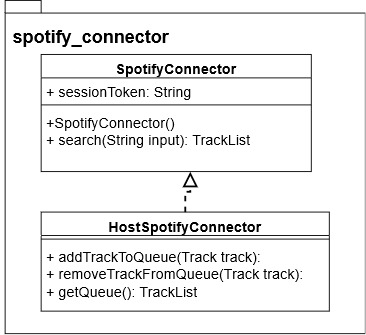
\includegraphics[width = 12cm]{LATEX/Entwurf/Graphics/spotify_connector.jpg}
\end{center}
\captionof{figure}{spotify\_connector uml-diagramm}


\subsubsection{class SpotifyConnector}
\textbf{attributes:}
\begin{itemize}
    \item authToken: String
    \begin{itemize}
        \item used to authenticate the request to spotify
    \end{itemize}
\end{itemize}


\subsection{user}

\subsubsection{class User}
\textbf{attributes:}
\begin{itemize}
    \item voteList: TrackList
    \begin{itemize}
        \item list of all tracks that can currently be voted on
    \end{itemize}
    \item blackList: TrackList
    \begin{itemize}
        \item list of all tracks that are currently blacklisted
    \end{itemize}
    \item cooldownList: TrackList
    \begin{itemize}
        \item list of all tracks that are currently on cooldown
    \end{itemize}
\end{itemize}
\textbf{constructors:}
\begin{itemize}
    \item User(Session session, BackendConnector backendConnector)
    \begin{itemize}
        \item assigns arguments to attributs.
    \end{itemize}
\end{itemize}
\textbf{methods:}
\begin{itemize}
    \item addTrackToVoteList(Track track)
    \begin{itemize}
        \item add track to VoteList
        \item calls backendConnector.addTrackToVoteList(track) to communicate change to the backend
    \end{itemize}
    \item requestStatistics()

    \item search(String input):
    \begin{itemize}
        \item searches the input in the VoteList and with spotifyConnector.search(input)
        \item validates the found tracks are not restricted by the session, with session.validateTrack(track)
        \item returns the found tracks as TrackList 
    \end{itemize}

    \item syncWithServer():
    \begin{itemize}
        \item calls backendConnector.syncwithServer() and assigns the returned TrackLists to the voteList, cooldownList and blackList
        \item after this method the state of user is in sync with the backend
    \end{itemize}
    
\end{itemize}


\subsubsection{class Host:}
Inherits from User, and adds methods specific to the Host role 
\textbf{attributes:}
\begin{itemize}
    \item queue: TrackList
    \begin{itemize}
        \item list of all tracks currently in the queue
    \end{itemize}
\end{itemize}
\textbf{constructors:}
\begin{itemize}
    \item Host(Session session, BackendConnector backendConnector, HostSpotifyConnector hostSpotifyConnector)
    \begin{itemize}
        \item calls super(session, hostBackendConnector,hostSpotifyConnector).
        \item The hostBackendConnector gets cast to BackendConnector, but can be cast back to HostBackendConnector instance at any time.
        \item The hostBackendConnector gets cast to SpotifyConnector, but can be cast back to HostSpotifyConnector instanceat any time.
        
    \end{itemize}
\end{itemize}
\textbf{methods:}
\begin{itemize}
    \item addTrackToQueue(Track track)
    \begin{itemize}
        \item adds track to this.queue 
        \item casts the spotifyConnector back to the hostSpotifyConnector.
        \item calls hostSpotifyConnector.addTrackToQueue(track) add the track to the spotify queue.
    \end{itemize}
    \item removeTrackFromQueue(Track track)
    \begin{itemize}
        \item remove track from this.queue 
        \item casts the spotifyConnector back to the hostSpotifyConnector.
        \item calls hostSpotifyConnector.removeTrackToQueue(track) to remove the track from the spotify queue.
    \end{itemize}
    \item addTrackToBlockList(Track track):
    \begin{itemize}
        \item adds track to this.blockList
        \item casts the backendConnector back to an hostBackendConnector
        \item call addTrackToBlockList(track) to mark the track as blocked in the backend.
    \end{itemize}
    \item removeTrackFromBlockList(Track track):
    \begin{itemize}
        \item remove track from this.blockList
        \item casts the backendConnector back to an hostBackendConnector
        \item call removeTrackFromBlockList(track) to mark the track as not blocked anymore in the backend.
    \end{itemize}
    \item syncWithQueue(): 
    \begin{itemize}
        \item casts SpotifyConnector back to hostSpotifyConnector
        \item cast backendConnector back to hostBackendConnector
        \item calls hostSpotifyConnector.getQueue() to get the current Queue from Spotify and compares it to this.queue
        \item if the first from this.queue is not present in the currentQueue from Spotify it has been played, its timestamp gets updated and it will get added to cooldownList. Additionally hostBackendConnector.addCooldownToTrack(track) gets called to communicate the change to the backend.
        \item update this.queue to the returned TrackList from the hostSpotifyConnector.getQueue()-call.
    \end{itemize}

\subsubsection{class FullParticant}:
Inherits from User, and adds methods specific to the FullParticant role 
\textbf{attributes}
\begin{itemize}
    \item none
\end{itemize}
\textbf{constructors:}
\item FullParticapant(Session session,ParticantBackendConnector particantBackendConnector,SpotifyConnector spotifyConnector) 
\begin{itemize}
    \item call super(session,particantBackendConnector,spotifyConnector)
    \item particantBackendConnector gets cast to instance of BackendConnector, but can be casted back to ParticantBackendConnector if required.
\end{itemize}
\textbf{methods}:
\begin{itemize}
    \item leaveSession():
    \begin{itemize}
        \item cast backendConnector back to particantBackendConnector()
        \item call particantBackendConnector.leaveSession()
    \end{itemize}
\end{itemize}

\subsubsection{class RestrictedParticant}:
Inherits from User, and adds methods specific to the FullParticant role 
\textbf{attributes}
\begin{itemize}
    \item none
\end{itemize}
\textbf{constructors:}
\item RestrictedParticapant(Session session,ParticantBackendConnector particantBackendConnector,SpotifyConnector spotifyConnector) 
\begin{itemize}
    \item call super(session,particantBackendConnector,spotifyConnector)
    \item particantBackendConnector gets cast to instance of BackendConnector, but can be casted back to ParticantBackendConnector if required.
\end{itemize}
\textbf{methods}:
\begin{itemize}
    \item search(String input): TrackList
    \begin{itemize}
        \item cast backendConnector back to particantBackendConnector()
        \item call particantBackendConnector.leaveSession()
    \end{itemize}
\end{itemize}


















\section{ViewModel}
\label{sec:App:ViewModel}

\section{View}
\label{sec:App:View}

\chapter{Server}
\label{chap:Server}

Der Server besteht aus einem Python Programm, welches eingehende Webrequests entgegen nimmt, diese verarbeitet und dann die entsprechenden Änderungen an der Datenbank vornimmt.

\section{API POST Requests}

Alle API Post Requests an den Server müssen an die f**olgende Adresse gesendet werden: "https://nep-tune.de:5000/[request]", wobei [request] den jeweiligen Typ der Request angibt.

Das Standartformat für alle Parameter einer Request ist JSON, hierbei soll folgender Header für die Request genutzt werden können: "Content-Type:application/json".

Das Standartformat für alle Rückgabewerte ist ebenfalls JSON.
Jeder Rückgabewert einer Request hat den Folgenden Aufbau: \{"status": ["success" | "failed"](str), ...\}, der Status indiziert ob der Aufruf der Request erfolgreich verlaufen ist oder nicht.

Im Fall dass der Aufruf nicht erfolgreich verlaufen ist, wird folgender Wert zurückgegeben: \{"status": "failed", "error": [error message](str)\}, die [error message] beschreibt hierbei den aufgetretenen Fehler und soll vor allem für Debugzwecke verwendet werden können.

TODO Flask erklären

\subsection{createNewSession}

This method creates a new session by calling the createNewSession method of the sessionHandler. It returns the sessionID and the timestamp of the session to the host.

\textbf{Parameters:}

\begin{itemize}
    \item \textbf{hostDeviceID} (str): The deviceID of the host.
    \item \textbf{modus} (str): The modus of the session. It is a set of "General", "Artist", "Genre", "Playlist".
    \item \textbf{cooldownTimer} (int): The cooldown timer of the session in minutes. It ranges from 0 to 720.
    \item \textbf{artists} (array[str]): All allowed artists of the session, only used in artistmode, otherwise null.
    \item \textbf{genres} (array[str]): All allowed genres of the session, only used in genremode, otherwise null.
    \item \textbf{playlist} (str): The URL for the standard fallback playlist of the session, if autoplay is preferred set to null.
\end{itemize}

\textbf{Returns:}

\begin{itemize}
    \item \textbf{sessionID} (int): The newly created sessionID. It ranges from 0 to 999999.
    \item \textbf{timestamp} (int): Timestamp the session was created at, for unique identification.
\end{itemize}

\textbf{Raises:}

\begin{itemize}
    \item \textbf{error} (sql error): If there is an error executing the SQL commands.
\end{itemize}


\subsection{deleteSession}

This method deletes a session by calling the deleteSession method of the sessionHandler. The sessionID is obtained from the userHandler by calling the getSessionIDByHostDeviceID method.

\textbf{Parameters:}

\begin{itemize}
    \item \textbf{hostDeviceID} (str): The deviceID of the host.
\end{itemize}

\textbf{Returns:}

\begin{itemize}
    \item None
\end{itemize}

\textbf{Raises:}

\begin{itemize}
    \item \textbf{error} (Session does not exist, or user is not host of the session): If the given user is not host of a session.
    \item \textbf{error} (sql error): If there is an error executing the SQL commands.
\end{itemize}


\subsection{getUserSessionState}

This method returns the user is an active participant, host or not a member of a session, by calling the getSessionIDByParticipantDeviceID and getSessionIDByHostDeviceID methods of the userHandler.

\textbf{Parameters:}

\begin{itemize}
    \item \textbf{deviceID} (str): The deviceID of the user.
\end{itemize}

\textbf{Returns:}

\begin{itemize}
    \item \textbf{userSessionState} (str (set("NONE", "PARTICIPANT", "HOST"))): The userSessionState of the user.
\end{itemize}

\textbf{Raises:}

\begin{itemize}
    \item \textbf{error} (sql error): If there is an error executing the SQL commands.
\end{itemize}


\subsection{getAllTrackData}

This method returns all tracks of the session, by calling the getTracksBySessionID method of the trackHandler. The locked tracks are obtained by calling the getLockedTracks method of the trackHandler.

\textbf{Parameters:}

\begin{itemize}
    \item \textbf{deviceID} (str): The deviceID of the user.
\end{itemize}

\textbf{Returns:}

\begin{itemize}
    \item \textbf{tracks} (array[track]): All tracks of the session.
    \item \textbf{lockedTracks} (array[trackID]): The ID of all locked tracks of the session.
\end{itemize}

\textbf{Raises:}

\begin{itemize}
    \item \textbf{error} (sql error): If there is an error executing the SQL commands.
\end{itemize}


\subsection{getStatistics}

This method returns the most upvoted song, genre and artist, the total played tracks, the session duration, the total participants and the total upvotes of the session, by calling the getSessionStatsBySessionID method of the sessionHandler.

\textbf{Parameters:}

\begin{itemize}
    \item \textbf{deviceID} (str): The deviceID of the user.
\end{itemize}

\textbf{Returns:}

\begin{itemize}
    \item \textbf{mostUpvotedSong} (str): The most upvoted song of the session.
    \item \textbf{mostUpvotedGenre} (str): The most upvoted genre of the session.
    \item \textbf{mostUpvotedArtist} (str): The most upvoted artist of the session.
    \item \textbf{totalPlayedTracks} (int): The total played tracks of the session.
    \item \textbf{sessionDuration} (str): The session duration of the session.
    \item \textbf{totalParticipants} (int): The total participants of the session.
    \item \textbf{totalUpvotes} (int): The total amount of upvotes of the session.
\end{itemize}

\textbf{Raises:}

\begin{itemize}
    \item \textbf{error} (sql error): If there is an error executing the SQL commands.
\end{itemize}


\subsection{participantJoinSession}

The method adds a participant to a session by calling the participantJoinSession method of the userHandler. The timestamp, modus, artists and genres of the session are obtained by calling the getSessionInfoBySessionID method of the sessionHandler.

\textbf{Parameters:}

\begin{itemize}
    \item \textbf{participantDeviceID} (str): The deviceID of the participant.
    \item \textbf{sessionID} (int (min 0, max 999999)): The ID of the session.
\end{itemize}

\textbf{Returns:}

\begin{itemize}
    \item \textbf{timestamp} (int): timestamp the session was created at, for unique identification.
    \item \textbf{modus} (str (set("General", "Artist", "Genre", "Playlist"))): The modus of the session.
    \item \textbf{artists} (array[str]): All allowed artists of the session, only used in artistmode, otherwise null.
    \item \textbf{genres} (array[str]): All allowed genres of the session, only used in genremode, otherwise null.
\end{itemize}

\textbf{Raises:}

\begin{itemize}
    \item \textbf{error} (Participant is already in a session): If the given participant is already in a session.
    \item \textbf{error} (Session does not exist): If the given session does not exist.
    \item \textbf{error} (sql error): If there is an error executing the SQL commands.
\end{itemize}


\subsection{participantLeaveSession}

The method sets a participant to inactive by calling the participantLeaveSession method of the userHandler.

\textbf{Parameters:}

\begin{itemize}
    \item \textbf{participantDeviceID} (str): The deviceID of the participant.
\end{itemize}

\textbf{Returns:}

\begin{itemize}
    \item None
\end{itemize}

\textbf{Raises:}

\begin{itemize}
    \item \textbf{error} (Participant is not in a session): If the given participant is not in a session.
    \item \textbf{error} (sql error): If there is an error executing the SQL commands.
\end{itemize}


\subsection{isSessionOpen}

The method checks if the session is still open by comparing the timestamp of the session with the timestamp of the request.

\textbf{Parameters:}

\begin{itemize}
    \item \textbf{sessionID} (int (min 0, max 999999)): The ID of the session.
    \item \textbf{timestamp} (int): timestamp the session was created at, for unique identification.
\end{itemize}

\textbf{Returns:}

\begin{itemize}
    \item \textbf{isOpen} (boolean): True if the session is still open, False otherwise.
\end{itemize}

\textbf{Raises:}

\begin{itemize}
    \item \textbf{error} (sql error): If there is an error executing the SQL commands.
\end{itemize}


\subsection{addTrackToSession}

The method adds a track to the session by calling the addTrackToSession method of the trackHandler.

\textbf{Parameters:}

\begin{itemize}
    \item \textbf{deviceID} (str): The deviceID of the user.
    \item \textbf{trackID} (str): The ID of the track.
    \item \textbf{trackName} (str): The name of the track.
    \item \textbf{artist} (array[str]): The artists of the track.
    \item \textbf{genre} (array[str]): The genres of the track.
    \item \textbf{imageURL} (str): The image URL of the track.
\end{itemize}

\textbf{Returns:}

\begin{itemize}
    \item None
\end{itemize}

\textbf{Raises:}

\begin{itemize}
    \item \textbf{error} (sql error): If there is an error executing the SQL commands.
\end{itemize}


\subsection{addUpvoteToTrack}

The method adds an upvote to a track by calling the addVotesToTrack method of the trackHandler.

\textbf{Parameters:}

\begin{itemize}
    \item \textbf{deviceID} (str): The deviceID of the user.
    \item \textbf{trackID} (str): The ID of the track.
\end{itemize}

\textbf{Returns:}

\begin{itemize}
    \item None
\end{itemize}

\textbf{Raises:}

\begin{itemize}
    \item \textbf{error} (sql error): If there is an error executing the SQL commands.
\end{itemize}


\subsection{removeUpvoteFromTrack}

The method removes an upvote from a track by calling the addVotesToTrack method of the trackHandler.

\textbf{Parameters:}

\begin{itemize}
    \item \textbf{deviceID} (str): The deviceID of the user.
    \item \textbf{trackID} (str): The ID of the track.
\end{itemize}

\textbf{Returns:}

\begin{itemize}
    \item None
\end{itemize}

\textbf{Raises:}

\begin{itemize}
    \item \textbf{error} (sql error): If there is an error executing the SQL commands.
\end{itemize}


\subsection{playedTrack}

The method resets the upvotes of a track, increments the total played tracks of the session and sets the cooldown start of the track to the current time, by calling the playedTrack method of the trackHandler.

\textbf{Parameters:}

\begin{itemize}
    \item \textbf{deviceID} (str): The deviceID of the user.
    \item \textbf{trackID} (str): The ID of the track.
\end{itemize}

\textbf{Returns:}

\begin{itemize}
    \item None
\end{itemize}

\textbf{Raises:}

\begin{itemize}
    \item \textbf{error} (sql error): If there is an error executing the SQL commands.
\end{itemize}


\subsection{setBlockTrack}

The method sets the blocked status of a track, by calling the setBlockTrack method of the trackHandler.

\textbf{Parameters:}

\begin{itemize}
    \item \textbf{hostDeviceID} (str): The deviceID of the host.
    \item \textbf{trackID} (str): The ID of the track.
    \item \textbf{blocked} (boolean): The blocked status of the track.
\end{itemize}

\textbf{Returns:}

\begin{itemize}
    \item None
\end{itemize}

\textbf{Raises:}

\begin{itemize}
    \item \textbf{error} (sql error): If there is an error executing the SQL commands.
\end{itemize}


\subsection{getLockedTracks}

The method returns the ID of all locked tracks of the session, by calling the getLockedTracks method of the trackHandler.

\textbf{Parameters:}

\begin{itemize}
    \item \textbf{deviceID} (str): The deviceID of the user.
\end{itemize}

\textbf{Returns:}

\begin{itemize}
    \item \textbf{lockedTracks} (array[str]): The ID of all locked tracks of the session.
\end{itemize}

\textbf{Raises:}

\begin{itemize}
    \item \textbf{error} (sql error): If there is an error executing the SQL commands.
\end{itemize}

\section{Database SQL Requests}

Die Mathoden, welche SQL Requests an die Datenbank schicken sind in drei Klassen aufgeteilt.


TODO MariaDBConnector erklären.

\subsection{sessionHandler}

\subsubsection{createNewSession}

This function creates a new session and returns the sessionID and the timestamp of the session. First a random sessionID is generated until an unused one is found. Then all session data is written to the database.

\textbf{Parameters}

\begin{itemize} \item \textbf{hostDeviceID} (int): The deviceID of the host. \item \textbf{modus} (int): The modus of the session. \item \textbf{cooldownTimer} (int): The cooldown timer of the session. \item \textbf{artists} (list): The artists of the session. \item \textbf{genres} (list): The genres of the session. \item \textbf{playlist} (list): The playlist of the session. \end{itemize}

\textbf{Returns}

\begin{itemize} \item \textbf{sessionID} (int): The ID of the session. \item \textbf{timestamp} (int): timestamp the session was created at. \end{itemize}

\textbf{Raises}

\begin{itemize} \item \textbf{mariadb.Error}: If there is an error executing the SQL commands. \end{itemize}

\subsubsection{deleteSession}

This function deletes the session with the given sessionID. First the session is deleted from the database. Then all participants are removed from the session. Then all tracks are removed from the session. If a track is not in any session anymore, it is removed from the global genre and artist list.

\textbf{Parameters}

\begin{itemize} \item \textbf{sessionID} (int): The ID of the session. \end{itemize}

\textbf{Returns}

\begin{itemize} \item None \end{itemize}

\textbf{Raises}

\begin{itemize} \item \textbf{mariadb.Error}: If there is an error executing the SQL commands. \end{itemize}

\subsubsection{getTimestampBySessionID}

This function returns the timestamp of the session with the given sessionID.

\textbf{Parameters}

\begin{itemize} \item \textbf{sessionID} (int): The ID of the session. \end{itemize}

\textbf{Returns}

\begin{itemize} \item \textbf{timestamp} (int): The timestamp of the session, or -1 if the session does not exist. \end{itemize}

\textbf{Raises}

\begin{itemize} \item \textbf{mariadb.Error}: If there is an error executing the SQL commands. \end{itemize}

\subsubsection{getSessionInfoBySessionID}

This function returns the modus, artists and genres of the session with the given sessionID. The artists and genres are returned as lists.

\textbf{Parameters}

\begin{itemize} \item \textbf{sessionID} (int): The ID of the session. \end{itemize}

\textbf{Returns}

\begin{itemize} \item \textbf{modus} (int): The modus of the session. \item \textbf{artists} (list): The allowed artists of the session. \item \textbf{genres} (list): The allowed genres of the session. \end{itemize}

\textbf{Raises}

\begin{itemize} \item \textbf{mariadb.Error}: If there is an error executing the SQL commands. \end{itemize}


\subsubsection{getSessionStatsBySessionID}

This function returns the most upvoted song, genre and artist, the total played tracks, the session duration, the total participants and the total upvotes of the session with the given sessionID.

\textbf{Parameters}

\begin{itemize}
    \item \textbf{sessionID} (int): The ID of the session.
\end{itemize}

\textbf{Returns}

\begin{itemize}
    \item \textbf{mostUpvotedSong} (string): The ID of the most upvoted song of the session.
    \item \textbf{mostUpvotedGenre} (string): The most upvoted genre of the session.
    \item \textbf{mostUpvotedArtist} (string): The most upvoted artist of the session.
    \item \textbf{totalPlayedTracks} (int): The total amount of played tracks of the session.
    \item \textbf{sessionDuration} (int): The duration of the session in minutes.
    \item \textbf{totalParticipants} (int): The total amount of participants of the session.
    \item \textbf{totalUpvotes} (int): The total amount of upvotes of the session.
\end{itemize}

\textbf{Raises}

\begin{itemize}
    \item \textbf{mariadb.Error}: If there is an error executing the SQL commands.
\end{itemize}



\subsection{userHandler}

\subsubsection{participantJoinSession}

This function adds the participant to the session if he is not already in it. If the participant was before in the session, he is set to active.

\textbf{Parameters}

\begin{itemize}
    \item \textbf{participantID} (int): The ID of the participant.
    \item \textbf{sessionID} (int): The ID of the session.
\end{itemize}

\textbf{Returns}

\begin{itemize}
    \item None
\end{itemize}

\textbf{Raises}

\begin{itemize}
    \item \textbf{mariadb.Error}: If there is an error executing the SQL commands.
\end{itemize}

\subsubsection{participantLeaveSession}

This function removes the participant from the session that he is currently in. If the participant is not in a session, nothing happens.

\textbf{Parameters}

\begin{itemize}
    \item \textbf{participantID} (int): The ID of the participant.
\end{itemize}

\textbf{Returns}

\begin{itemize}
    \item None
\end{itemize}

\textbf{Raises}

\begin{itemize}
    \item \textbf{mariadb.Error}: If there is an error executing the SQL commands.
\end{itemize}

\subsubsection{getSessionIDByParticipantDeviceID}

This function returns the sessionID if the given user is active participant of a session, -1 otherwise.

\textbf{Parameters}

\begin{itemize}
    \item \textbf{participantID} (int): The ID of the participant.
\end{itemize}

\textbf{Returns}

\begin{itemize}
    \item \textbf{sessionId} (int): The ID of the session, -1 if the participant is not in an active session.
\end{itemize}

\textbf{Raises}

\begin{itemize}
    \item \textbf{mariadb.Error}: If there is an error executing the SQL commands.
\end{itemize}

\subsubsection{getSessionIDByHostDeviceID}

This function returns the sessionID if the given user is host of a session, -1 otherwise.

\textbf{Parameters}

\begin{itemize}
    \item \textbf{hostDeviceID} (int): The ID of the host.
\end{itemize}

\textbf{Returns}

\begin{itemize}
    \item \textbf{sessionId} (int): The ID of the session, -1 if the host is not in a session.
\end{itemize}

\textbf{Raises}

\begin{itemize}
    \item \textbf{mariadb.Error}: If there is an error executing the SQL commands.
\end{itemize}

\subsubsection{getSessionIDByDeviceID}

This function returns the sessionID if the given user is host or active participant of a session, -1 otherwise.

\textbf{Parameters}

\begin{itemize}
    \item \textbf{userDeviceID} (int): The ID of the user.
\end{itemize}

\textbf{Returns}

\begin{itemize}
    \item \textbf{sessionId} (int): The ID of the session, -1 if the user is not in a session.
\end{itemize}



\subsection{trackHandler}

\subsubsection{getTracksBySessionID}

This function returns the trackID, trackName, upvotes, artists and imageURL of all tracks in the session. The artists are returned as a list.

\textbf{Parameters}

\begin{itemize} \item \textbf{sessionID} (int): The ID of the session. \end{itemize}

\textbf{Returns}

\begin{itemize} \item \textbf{tracklist} (list(tracks)): The list of tracks in the session. \end{itemize}

\textbf{Raises}

\begin{itemize} \item \textbf{mariadb.Error}: If there is an error executing the SQL commands. \end{itemize}

\subsubsection{addTrackToSession}

This function adds a track to the session, if it is not already in the session. The artists and genres are added to the global artist and genre list, if they are not already in the list.

\textbf{Parameters}

\begin{itemize} \item \textbf{sessionID} (int): The ID of the session. \item \textbf{trackID} (int): The ID of the track. \item \textbf{trackName} (string): The name of the track. \item \textbf{artists} (list(string)): The list of artists of the track. \item \textbf{genres} (list(string)): The list of genres of the track. \item \textbf{imageURL} (string): The URL of the image of the track. \end{itemize}

\textbf{Returns}

\begin{itemize} \item None \end{itemize}

\textbf{Raises}

\begin{itemize} \item \textbf{mariadb.Error}: If there is an error executing the SQL commands. \end{itemize}

\subsubsection{addVotesToTrack}

This function adds the given amount of upvotes to a track. If the amount of upvotes is negative, the upvotes are subtracted.

\textbf{Parameters}

\begin{itemize} \item \textbf{sessionID} (int): The ID of the session. \item \textbf{trackID} (int): The ID of the track. \item \textbf{amount} (int): The amount of upvotes to add. \end{itemize}

\textbf{Returns}

\begin{itemize} \item None \end{itemize}

\textbf{Raises}

\begin{itemize} \item \textbf{mariadb.Error}: If there is an error executing the SQL commands. \end{itemize}

\subsubsection{playedTrack}

This function sets the upvotes of the track to the given trackID to 0, sets the cooldown start of the track to the current time and increments the amount played of the track by one.

\textbf{Parameters}

\begin{itemize} \item \textbf{sessionID} (int): The ID of the session. \item \textbf{trackID} (int): The ID of the track. \end{itemize}

\textbf{Returns}

\begin{itemize} \item None \end{itemize}

\textbf{Raises}

\begin{itemize} \item \textbf{mariadb.Error}: If there is an error executing the SQL commands. \end{itemize}

\subsubsection{setBlockTrack}

This function sets the blocked status of the track to the given trackID to the given status.

\textbf{Parameters}

\begin{itemize} \item \textbf{sessionID} (int): The ID of the session. \item \textbf{trackID} (int): The ID of the track. \item \textbf{blocked} (boolean): The blocked status of the track. \end{itemize}

\textbf{Returns}

\begin{itemize} \item None \end{itemize}

\textbf{Raises}

\begin{itemize} \item \textbf{mariadb.Error}: If there is an error executing the SQL commands. \end{itemize}

\subsubsection{getLockedTracks}

This function returns all tracks that are blocked or on cooldown.

\textbf{Parameters}

\begin{itemize}
    \item \textbf{sessionID} (int): The ID of the session.
\end{itemize}

\textbf{Returns}

\begin{itemize}
    \item \textbf{lockedTracks} (list(int)): The list of trackIDs of the locked tracks.
\end{itemize}

\textbf{Raises}

\begin{itemize}
    \item \textbf{mariadb.Error}: If there is an error executing the SQL commands.
\end{itemize}





\chapter{Database}
\label{chap:Database}

\chapter{Sequence diagrams}
\label{chap:Sequence diagrams}

\chapter{Glossary}
\label{chap:Glossary}

\end{document}
